\chapter{Hardware and Software Activities}
\label{chap:Hardware}

The Hadron Outer (HO) calorimeter of the CMS detector has been installed to measure the energy which is not contained by the barrel calorimeters. The HO improves the energy resolution of highly energetic hadrons and hence provide a better jet energy reconstruction as well as missing transverse energy resolution. HO is situated in the barrel return yokes (YB) in front of the first layer of muon chambers. The YBs consist of 5 rings of iron: YB0, YB$\pm$1 and YB$\pm$2. Rings R0, R$\pm$1 and R$\pm$2 of the HO system are located in YB0, YB$\pm$1 and YB$\pm$2 respectively. In the original design of HO, the signals of the detector were read out by hybrid photo-diodes (HPDs) by converting the wavelength shifted scintillator light into electrical charges. The electronics readout system of the HO is built using the 18-channel readout modules (RMs). The RMs combine the photo-sensors, amplifiers and analogue to digital converters (ADC) and are housed in crates (RBX). The newly developed SiPM system consists of three circuit boards : a mounting Board (MB) holding the SiPM, a bias board generating the SiPM operation voltage and the a control board connecting the SiPMs electrically to the HCAL readout electronics and monitors the operation of the individual SiPMs. The array of 18 SiPMs is mounted on one side of the MB. The geometrical constraints required a total of 132 RMs to read all channels. The HPDs were chosen as photo-sensors due to its high gain and magnetic field tolerance. But in Run I conditions of the CMS, HPDs proved to be less optimal because of the discharge caused by the fringe field of the CMS magnet, low gain and photo detection efficiency, and ageing effects. Due to these inefficiencies, the HPDs needed to be replaced with multi-pixel Geiger-mode avalanche photo-diodes also known as silicon photo-multipliers (SiPMs). The SiPMs are preferred because of the magnetic field insensitivity, relatively high gain and high photon-detection efficiency. This replacement was carried out during the first LHC long shutdown (LS1) in 2013-2014 \cite{Lutz:2012yoa}, where the LHC was upgraded to higher luminosity (5 $\times$ 10$^{34} {\rm cm}^2 {\rm s}^{-1}$) and center-of-mass energy of proton-proton collisions was increased from 4 TeV to 6.5 TeV per beam. During this up-gradation, the replacement of HPDs took place in two steps : first the existing RMs with HPDs were taken out from the detector and then were rebuild with SiPMs. After verifying the working of the RMs, they were re-installed in the CMS detector. In collaboration with HO group of the CMS, we participated in the re-installation of the RMs with SiPMs in place of HPDs specially in the sectors YB\plusn 1 and YB\plusn 2 of HCAL during the visits to CERN in March-April, 2014.

\section{Silicon Photo-Multipliers}
A silicon photo-multiplier (SiPM) used in HO is a Hamamatsu Multi-Pixel Photon Counter (MPPC) in a surface mounted device housing. It has a cell pitch of 50 $\micro$m with an active area of 3 $\times$ 3 mm. The required operating voltage required is $\sim$ 70 V with a gain $\sim$ 6 $\times$ 10$^5$ fC/photo-electron when operated at a voltage greater than the breakdown voltage by 1 V. At this over-voltage given by the bias voltage subtracted from the breakdown voltage, the typical dark current rate is of the order of a few hundred kHz. Along with the installation of SiPMs, the commissioning of the upgraded parts also took place. The commissioning includes the quickly identification of the problems with the new and existing hardware, validation of the installation and repairs, in case of any malfunctions, during the access to the hardware. To monitor and optimize the operational parameters, two types of the data were used : the signals from SiPMs in the absence of light referred as pedestal events (PED) and the charge distributions collected by illuminating the SiPMs with a calibrated light emitting diodes referred as LED events. While performing the Quality Control (QC) analysis, the PED and LED events or runs were taken through an online software created by HO CMS group. These runs were used to study and analyze the properties of SiPMs. 

In the first step of commissioning, a communication test was performed with the readout system along with the verification of slow control operation and channel response. After that, the measurements and optimization of SiPM operational variables were carried out. One of the important quantities of the SiPMs to study is the change of breakdown voltage (BV) and calibration factor gain (G) with the temperature. BV gives the threshold voltage after which the diodes switch to avalanche mode and gain corresponds to the charge produced by SiPM for a single photo-electron (SPE). The gain of SiPMs depends linearly on the temperature with a relative dependence of 8\% gain shift per K at an operating point of 1.5 V over-voltage \cite{Anderson:2011zzc}. As the gain depends linearly on the over-voltage, the change of the breakdown voltage with temperature translates into a change of the gain with temperature. This dependence requires an active control of the temperature of SiPMs with better than 0.1 K stability. So a peltier element is mounted on the back of the MB for cooling purposes in order to stabilize the temperature. We mainly studied the variations of BV and gain with temperature : \\ \newline
{\bf Breakdown Voltage -} The BV can be determined either by using the pedestal spectrum of the SiPMs or the signal of a short LED pulse. In the first method, the gain is estimated by performing a scan of the bias voltage. The dependence of the measured gain on the bias voltage is fitted with a linear function. The extrapolation of fit function to zero gain gives the value of the breakdown voltage. The second method uses the relative change of the measured signal (S) when pulsing an LED and varying the bias voltage (V). The distribution of dS/SdV as a function of V whose maximum provides the BV. This distribution is fitted by a simple Gaussian function to obtain the value of BV. The variation of the breakdown voltage, obtained using the LED method, over time is shown for one RM (18 channels) in Fig.~\ref{fig:BV}. When the detector is operated in stable conditions, it is observed that the BV measurements also stay stable within 50 mV which illustrate the reliability of the BV determination. This variation is studied over a period from the end of January, 2014 to the beginning of March, 2014 which indicates that if any changes are observed in gain or breakdown voltage, they are not caused by changes in the temperature.\\ \newline
\begin{figure}[!h]
\begin{center}
\vspace*{-10mm}
\hspace*{-5mm}
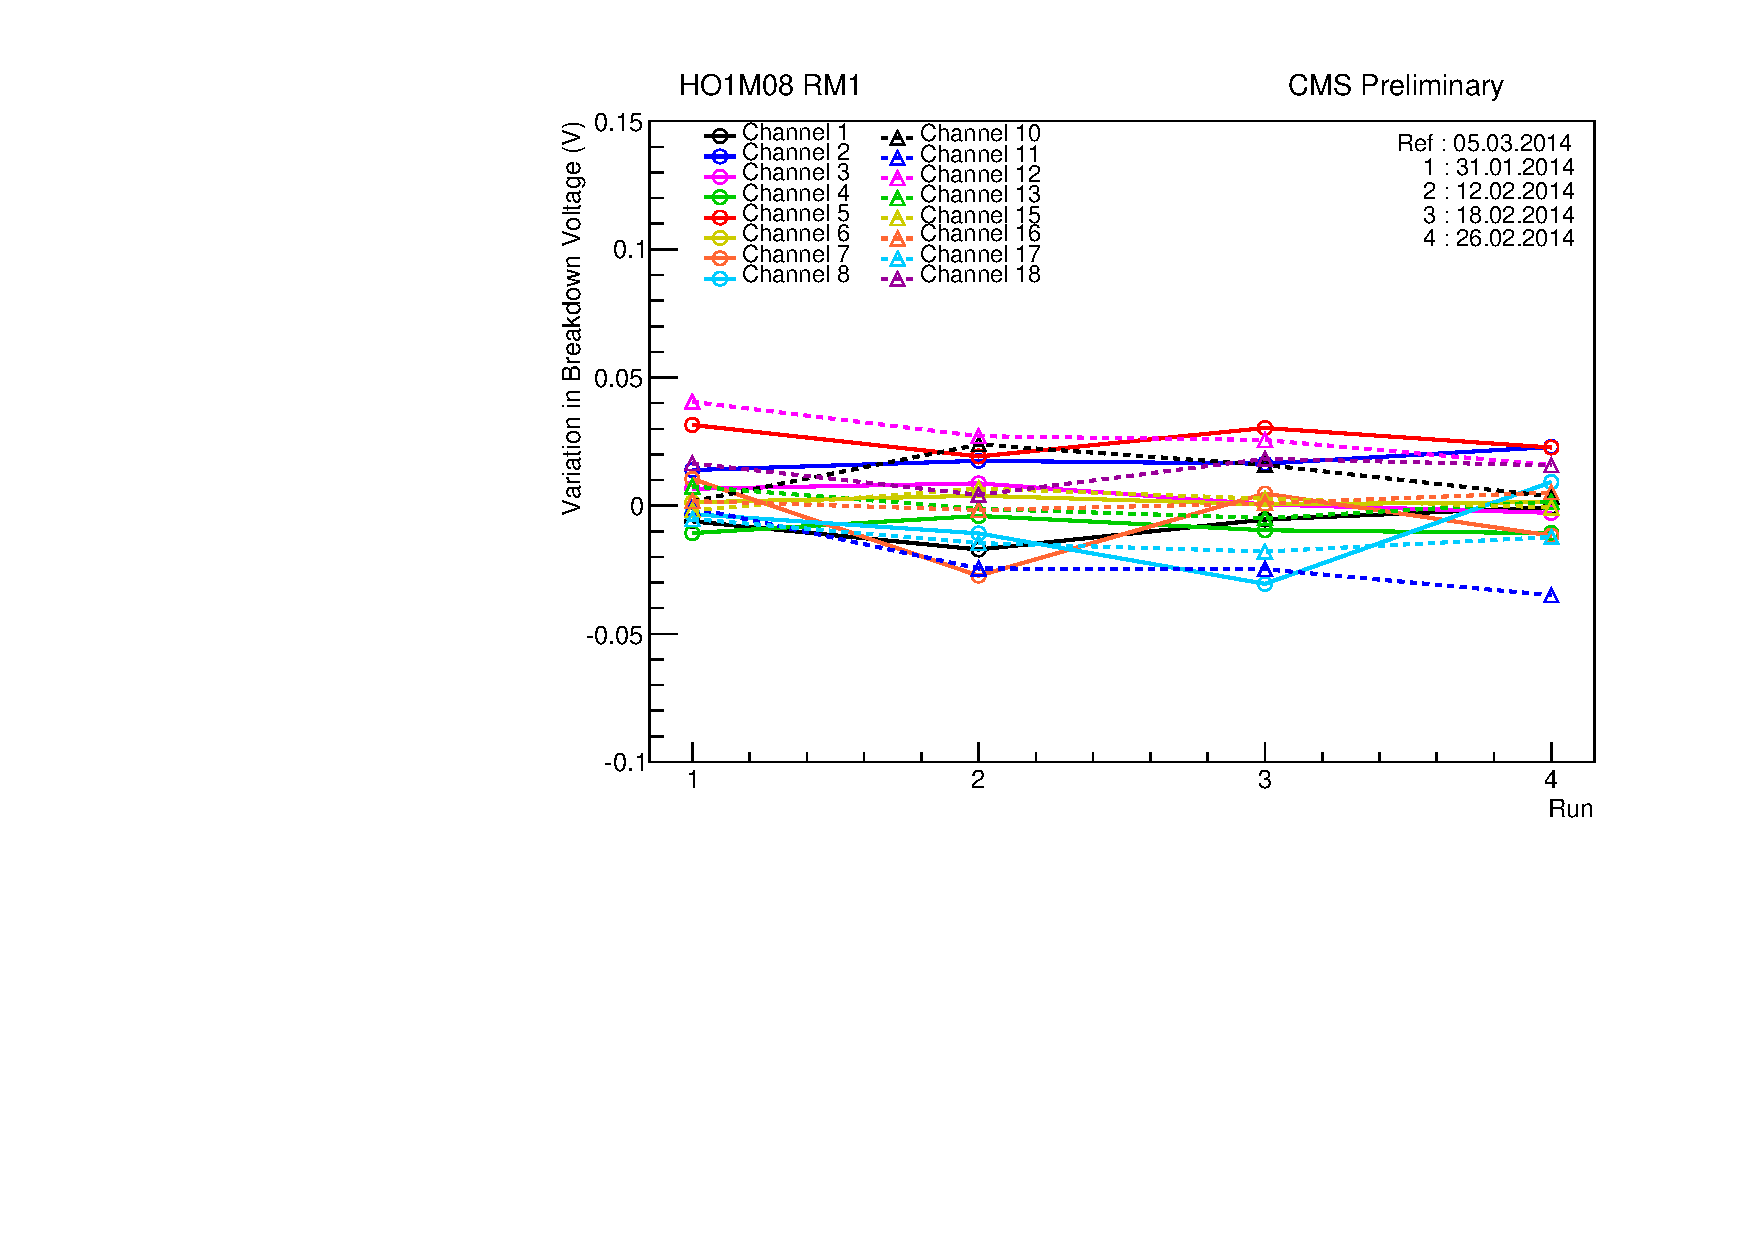
\includegraphics[scale = 0.65]{/home/anter/Desktop/Thesis/Figures/Final/bv_led_iv_49.pdf}\\
\vspace*{4mm}
\caption[The breakdown voltage (BV) is estimated using LED method and its variation is shown over time for 18 channels of one readout module (RM).]{The breakdown voltage (BV) is estimated using LED method and its variation is shown over time for 18 channels of one readout module (RM). When the detector is operated in stable conditions, the BV measurements also are stable within 50 mV illustrating the reliability of the BV determination.}
\label{fig:BV}
\end{center}
\end{figure} \newline
{\bf Gain -} The gain is determined by generating short light pulses with an LED onto the SiPM. Assuming the intensity of the light pulse not too large and $N$ as number of photons reaching the SiPM, the signal should be equal to $N \times$ gain. According to Poisson statistics, the sigma of the photon number is $\sqrt{N}$ and the sigma of the measured signal is $\sqrt{N} \times$ gain. Dividing the variance of the signal by the mean of the signal one gets sigma$^2$/mean = gain. Figure~\ref{fig:gain1} shows the relative variation of the gain versus time for a single SiPM mounting board. We observed that gain is stable over a time from the middle of February to the beginning of March in 2014 and the relative variation of the gain lies within 2\%. 
\begin{figure}[!h]
\begin{center}
\vspace{-2mm}
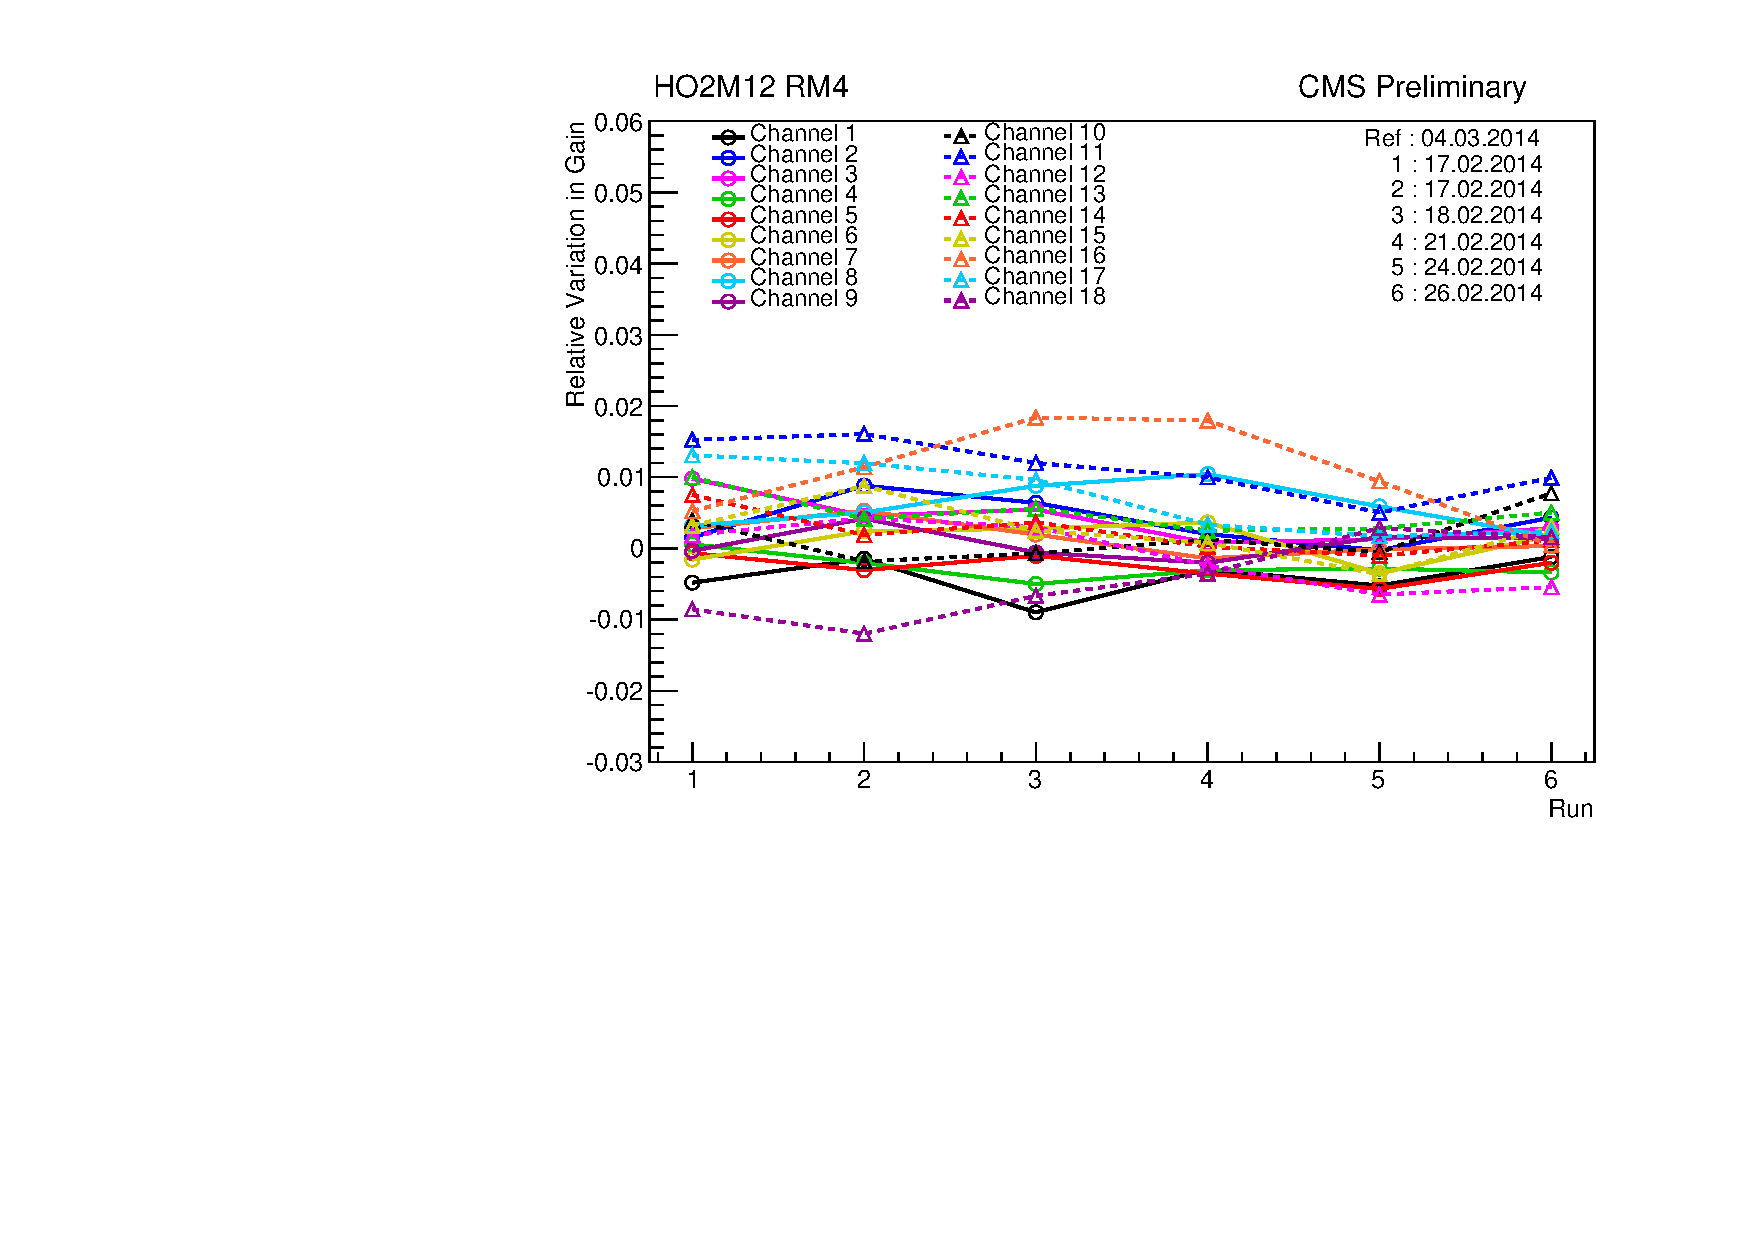
\includegraphics[scale = 0.65]{/home/anter/Desktop/Thesis/Figures/Final/Gain_PED_108.pdf}
\vspace*{4mm}
\caption{The relative variation of the SiPM gain is presented over time for a single RM with 18 channels. The gain is stable over a time from the middle of February to the beginning of March in 2014 and the relative variation of the gain lies within 2\%}
\label{fig:gain1}
\end{center}
\end{figure}\newline
The relative gain variation with time is plotted for all installed SiPMs as presented in Fig.~\ref{fig:gain2} which is fitted using a Gaussian function. The distribution has a width of only 0.5 \% and all gain variations are within 3\%. This illustrates that the gain determination behaves as expected and the operation of the SiPMs with a stable gain is possible. 
\begin{figure}[!h]
\begin{center}
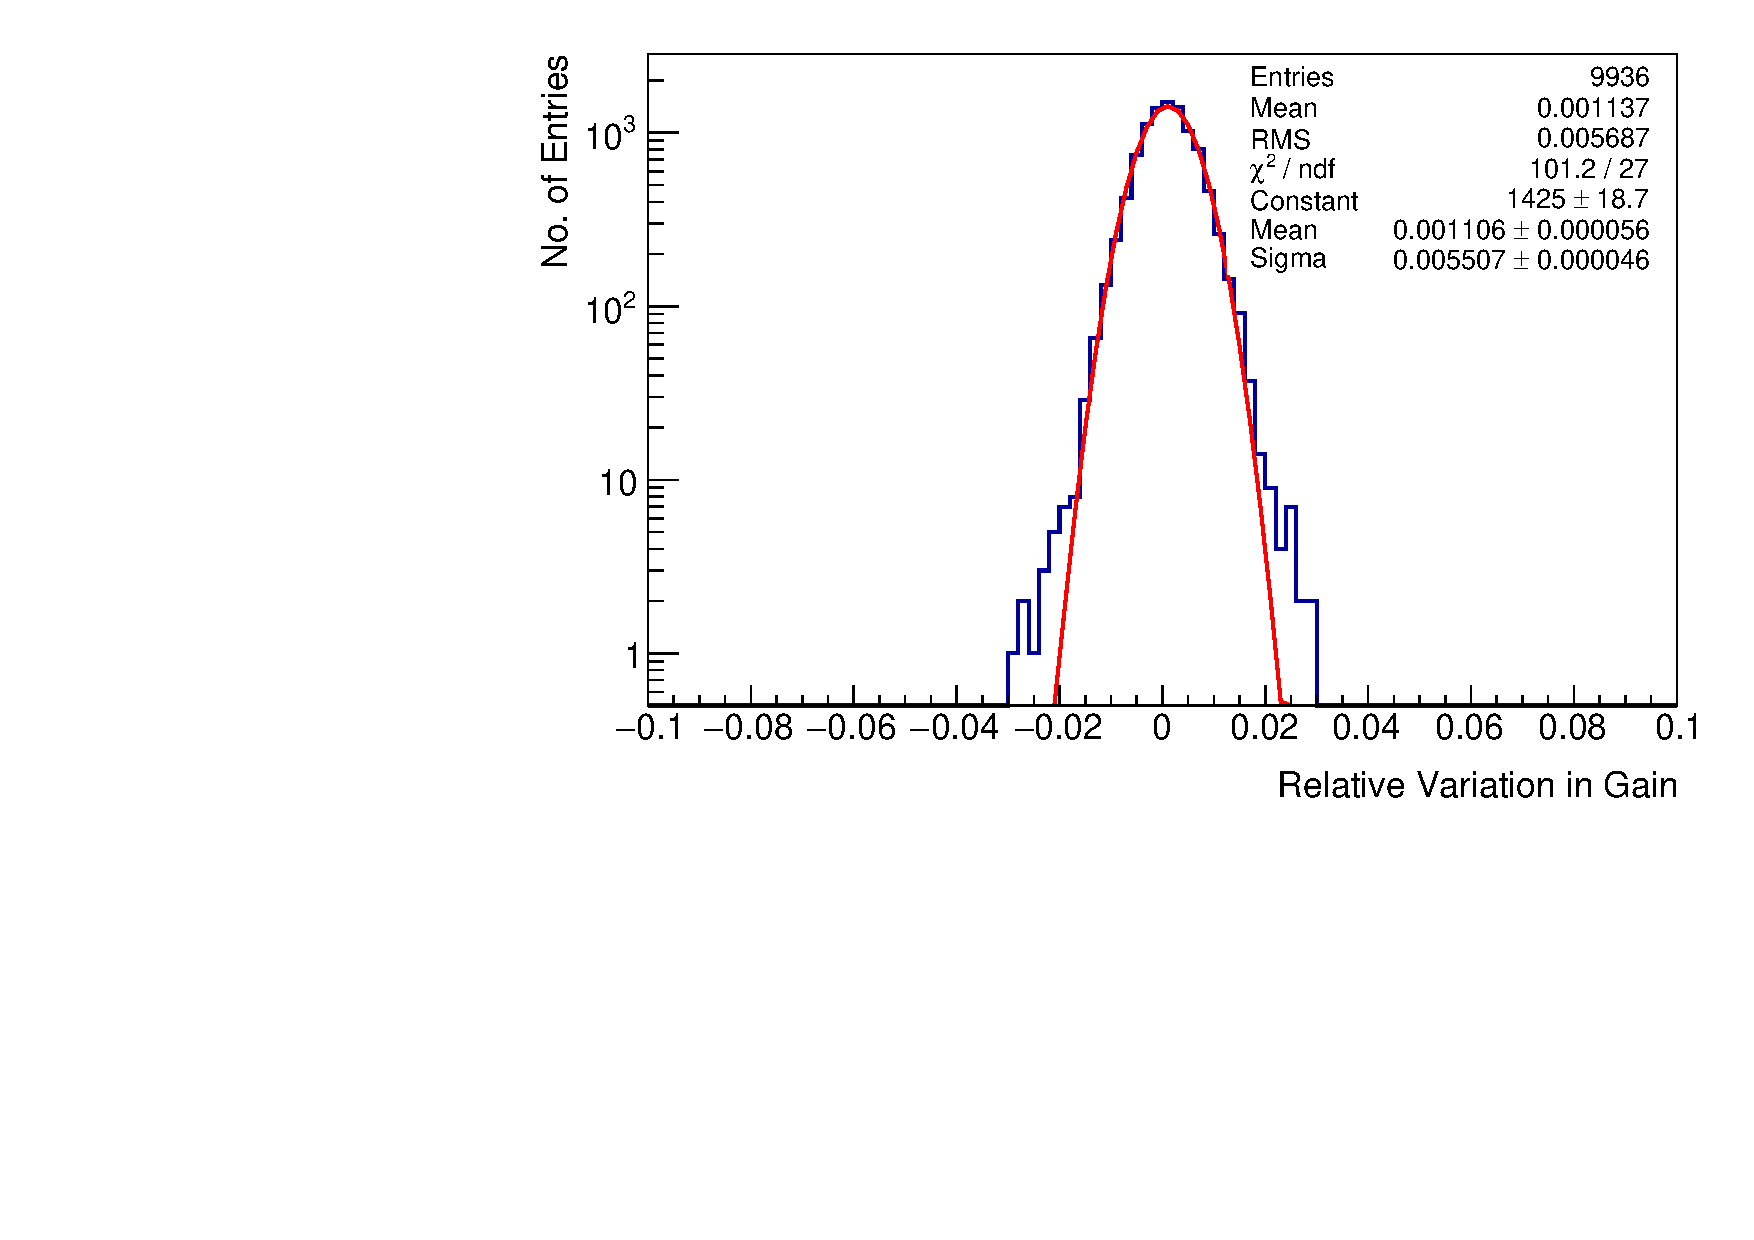
\includegraphics[scale = 0.6]{/home/anter/Desktop/Thesis/Figures/Final/Fit.pdf}
\vspace*{4mm}
\caption{The distribution of the relative variations in gain for all the installed SiPMs is fitted with a Gaussian function. It has a width of only 0.5 \% and all gain variations are within 3\%.}
\label{fig:gain2}
\end{center}
\end{figure}
These results were presented at the CALOR 2014 conference \cite{Kunsken:2015zla} and are documented in Ref. \cite{DN}.

\begin{figure}[!h]
\begin{center}
\vspace*{3mm} 
\hspace*{-5mm}
%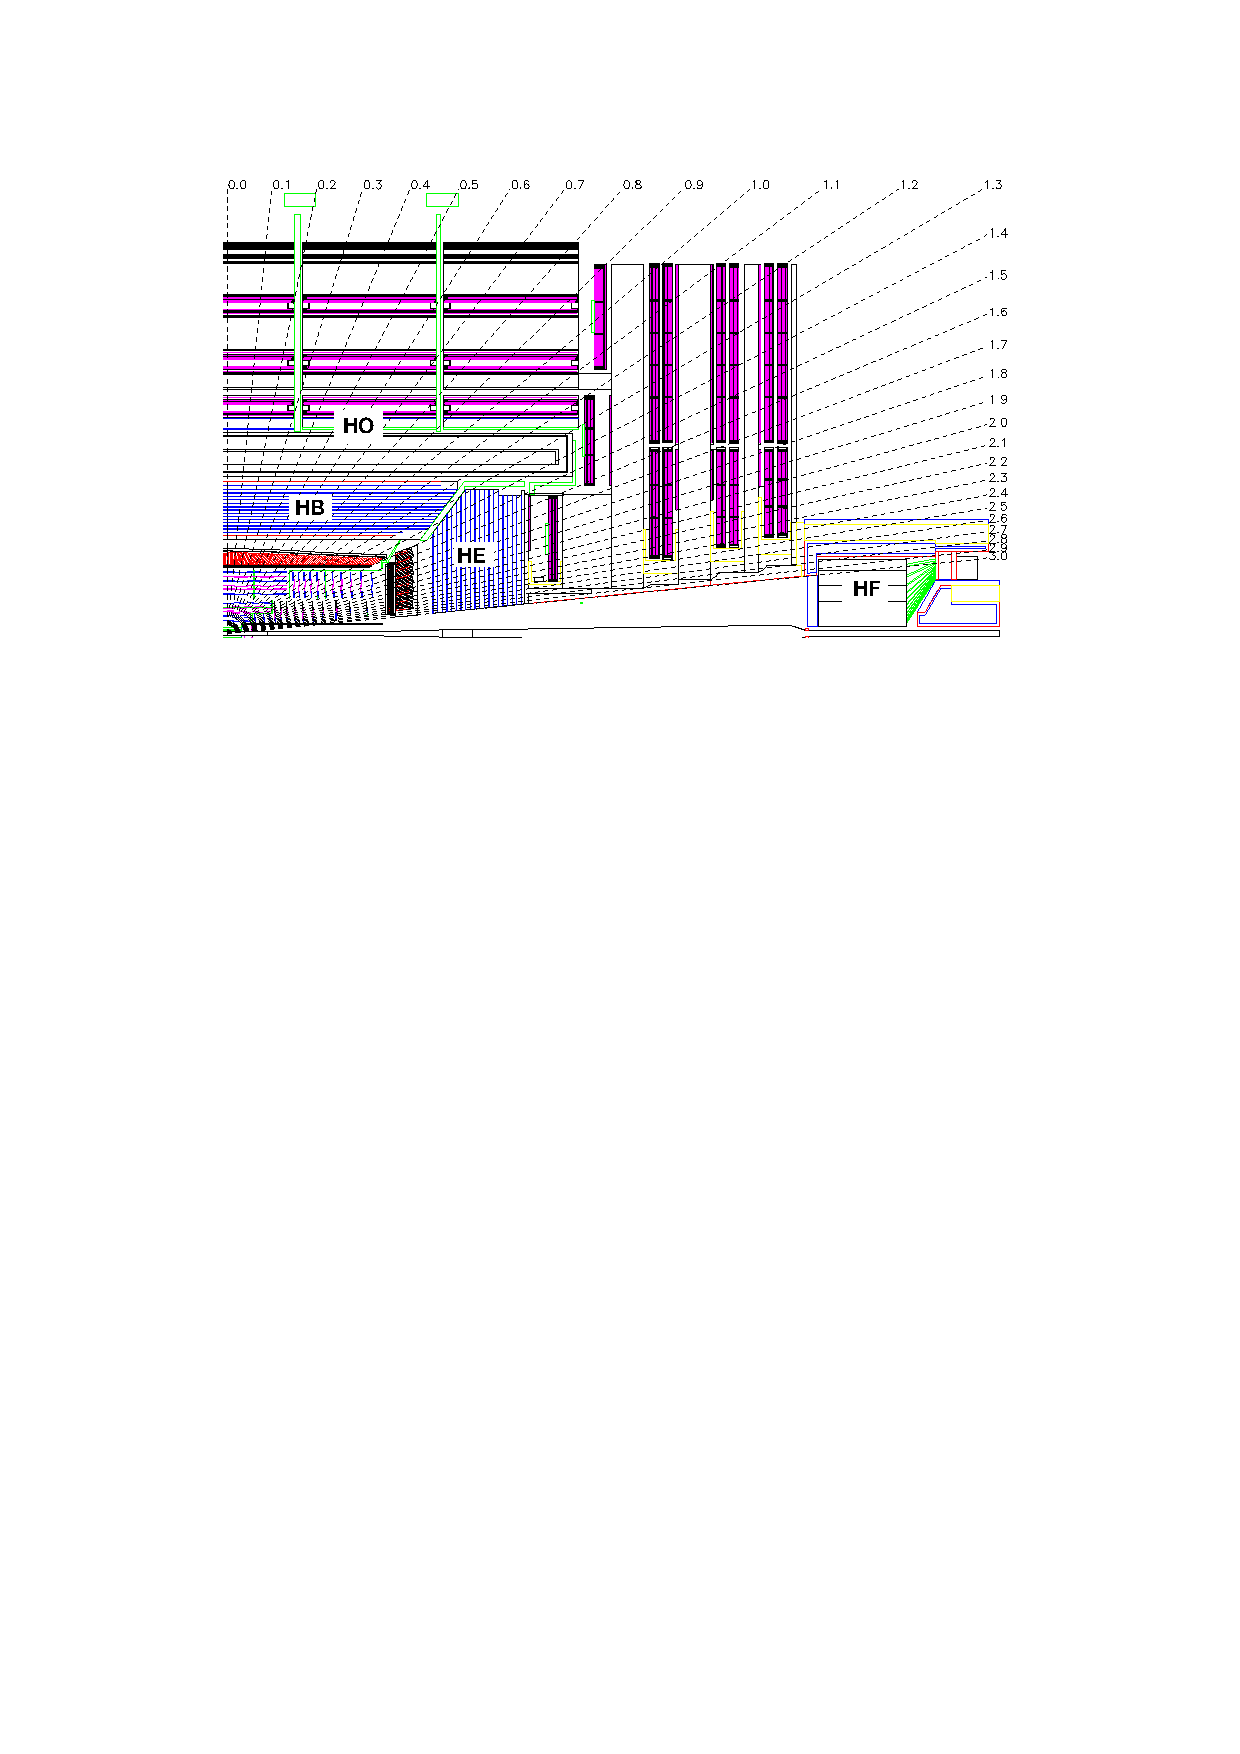
\includegraphics[scale = 1.]{/home/anter/Desktop/Thesis/Figures/edited_cropped_HCAL.pdf}\\
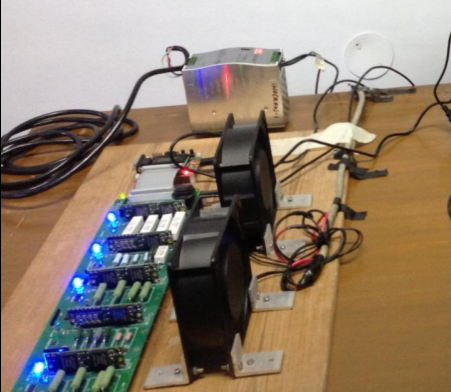
\includegraphics[scale = 0.8]{/home/anter/Desktop/Thesis/Figures/Final/Mezannine_3.png}\\
\vspace*{4mm}
\caption[Longitudinal section of one quarter of the hadronic calorimeter (HCAL) in $r$-$\eta$ plane.]{Longitudinal section of one quarter of the hadronic calorimeter (HCAL) in $r$-$\eta$ plane. It consists of different parts : hadron barrel (HB), hadron outer (HO), hadron endcap (HE) and hadron forward (HF). Taken from \cite{Chatrchyan:2008aa}.}
\label{fig:mez}
\end{center}
\end{figure}

\section{MicroTCA}
During the LHC upgrade at the time of LS1, the increase in LHC luminosity (and energy) increased the number of interactions per bunch crossing i.e. pileup. Hence, a large amount of the data became available which need to be processed at a much faster rate than before. This required an increase in the number of electronics readout channels to collect high quality data to perform physics analysis and a very high speed DAQ system. Before the upgrade, the VERSAbus Memory card (VME) based system was used which could not support data transfer rate needed after LS1. So during the upgradation, the existing VME based system was replaced with \mtca (Micro Telecommunications Computing Architecture) standard system in HCAL back-end electronics \cite{CMS:2012tda}. The \mtca is an embedded, scalable architecture which offers flexibility to build robust systems. It was designed as a complimentary system to the Advanced Telecommunication Computing Architecture (ATCA), primarily for the core telecommunication networks. It is compact in size and less expensive than ATCA systems. \mtca is based on the Advanced Mezzanine Card (AMC) standard which was part of the ATCA. The ATCA standard specifies a crate hosting a large carrier of AMC cards, also known as $\mu$HTR (Micro HCAL Trigger \& Readout) cards. In the simpler \mtca architecture, AMC cards are plugged directly into a backplane such that twelve standard AMC cards can be placed in a crate. One or two special hub slots are also present in each crate where at-least one of these slots must be occupied by a MicroTCA Carrier Hub (MCH) card. The MCH card is responsible for the control of the power to each slot and for general house-keeping of the crate.


A \mtca standard is made up of following interconnected elements : \\ \newline
{\bf Advanced Mezzanine Card (AMC) -} \\ \newline
{\bf Atleast one \mtca Carrier Hub (MCH) -} \\ \newline
{\bf The interconnect (backplane) -} \\ \newline
{\bf Power Modules -} \\ \newline
{\bf Cooling subsystem -} \\ \newline
{\bf Mechanical elements comprising a Shelf. -} \\ \newline


In \mtca, twelve \mhtr (HCAL Trigger/Readout) cards will receive the data links from the front-ends, calculate and transmit trigger primitives. Power Mezzanines/Auxiliary Power Mezzanines (PM/APM) mounted on \mhtr will supply power these cards. So, working of mezzanines becomes very crucial as there failure may lead to lose in the data collection efficiency.


One μT CA unit (crate) can hold upto 12 Advanced Mezzanine Cards (AMC), within CMS known
as micro HCAL Trigger \& Readout (μHT R Figure 2 right) card. It includes upto two special “hub”
slots. At least one of these slots must be occupied by a μT CA Carrier Hub (MCH) card which is
responsible for the control of the power to each slot and for general house-keeping of the crate. The
primary MCH site is to be used for a commercial MCH card responsible for crate management and the
Ethernet network. The secondary site is to be used for a CMS-common card which will be responsible
for clock and fast control distribution as well as local and global DAQ


– An apparatus shown in Figure 9 has been set up at Physics Department, Panjab University, Chandigarh to ensure the proper functioning of PM/APM. We successfully tested three sets of PM/APM, each set for 39 hours continuously.

● AMC:
The AMC standard defines a family of mezzanine cards that can be
used in a variety of ways. In a \mtca architecture, the AMC cards plug
directly into a backplane.
➢ Small size
➢ High speed connectivity
➢ Hot swappable
➢ Full management infrastructure


MCH:
A \mtca Carrier Hub is the main management module that enables and
controls different modules of the \mtca system. The MCH is responsible for the data
switching between the modules and provides the following features:
➢ Data connectivity to the AMCs
➢ Control and manage the AMCs, Power Modules and the Cooling Units
➢ Distribute clock signals to the AMCs
✔
✔
● Power
to various parts μHTR cards is supplied by Power
Mezzanines/Auxiliary Power Mezzanines (PM/APM).
● Working of mezzanines is very crucial as thir failure may lead to loss in
the data collection efficiency.
● Hence, a Power Mezzanine Testing program is designed to monitor or test
uHTR PM/APM for long term (~39 hour) stability tests.
The CMS Upgrade Working Group specifies a \mtca crate with two MCH sites and
up to twelve AMC slots.
One Commercial-MCH responsible for crate management and Ethernet
network.
A CMS-common MCH (AMC13) responsible for clock and fast control
distribution, local and global DAQ.
● Backplane:
A passive interface that provides the required data, management and
power connections to the \mtca modules. The Backplane along with the MCH
provides the virtual carrier interface to the AMCs.
➢ Direct point to point connections between AMCs
➢ MCH to AMC connections
● Power
Module: The Power Modules (PMs) are responsible for distribution and
management of power to various \mtca modules. PMs distribute two types of power
to the \mtca modules:
➢ +12 V power for module payload
➢ +3.3 V power for module management
➢ During
the test, PM/APM are inserted into the appropriate slots on test
board. The test is performed in four stages:
In addition, the PMs provide an interface to the MCH for power management. These
convert the incoming bulk -48 V DC power into 12 V DC for each slot.
● Cooling
Unit: The Cooling Units (CU) are essential to remove excess heat and
prevent damage to the modules. Cooling Units have intelligence and variable fan
speed support.
● FRU:
\mtca systems have several modules that can be added or removed in the
field known as Field Replaceable Units (FRU). The field replaceable units are AMC,
MCH, Power Modules and Cooling Units.


HCAL Trigger/Readout (μHTR) cards are responsible for:
Receiving the data links from the front-ends.
➢ Calculating and transmitting trigger primitives.
➢ Holding the Level 1 readout pipeline.


Transmitting and receiving ends.
➢ The μHTR cards will receive
data from the front-end electronics using PPOD-
type parallel optical receivers.


The μHTR contains two Virtex 6
➢ The FPGA which connects
Vadatech Crate VT892
Components
FPGAs.
directly to the front-end links is called the front
FPGA.
➢ One connecting directly to the DAQ and control links is called the back FPGA.
➢ The front FPGA connects directly to a PPOD parallel optical transmitter for
transmission of trigger primitives to the calorimeter trigger system.
➢ The front FPGA is responsible for sychronizing the data from all links,
calculating and transmitting the trigger primitives and holding the data pipeline
while waiting for the Level 1 decision.
➢ Once a Level 1 decision is issued the front FPGA transmits all the samples
associated with the event to the back FPGA.
➢ The back FPGA is responsible for buffering the data and performing zero-
suppression.

Power
to various parts μHTR cards is supplied by Power
Mezzanines/Auxiliary Power Mezzanines (PM/APM).
● Working of mezzanines is very crucial as thir failure may lead to loss in
the data collection efficiency.
● Hence, a Power Mezzanine Testing program is designed to monitor or test
uHTR PM/APM for long term (~39 hour) stability tests.


During
the test, PM/APM are inserted into the appropriate slots on test
board. The test is performed in four stages:

During
each test various parameters are taken care of and recorded after
every 10 seconds.
 Output voltage
 Current
 Power
 Temperature

As
a contribution to HCAL Back-end electronics upgrade, we participated
in the testing of PM/APM.
➢ To
ensure the proper functioning of PM/APM, 39 hours rigorous test
has to be performed.
➢ For this an apparatus has been set up at Physics Department, Panjab
University to carry out the testing procedure.
➢ We successfully tested three sets of PM/APM which were used for
μHTR cards.

Before
production, the back-end electronics (μHTR) will be the subject of a
specific electronics design review:

The
review will demonstrate that the designed electronics will meet the
requirements.
➢ The testing will validate the stable operation of the data links and
stable link latency on the front-end/back-end data link.
● As
a part of this testing of μHTR cards, a set-up has been installed at
Physics Department, Panjab University.


1. During upgradation of LHC, in HCAL Back-end electronics, the current VME (VERSAbus Memory card) based system was replaced with modern FPGAs and the \mtca (Micro Telecommunications Computing Architecture) based system to process large amount of the data. In \mtca, twelve \mhtr (HCAL Trigger/Readout) cards will receive the data links from the front-ends, calculate and transmit trigger primitives. A set-up for testing of \mhtr cards was installed at Department of Physics, Panjab University, Chandigarh and we successfully tested \mhtr cards. 

2. I was deputed to CERN from 9th February, 2015 to 7th May, 2015. I took 2 DQM (Data Quality Monitoring) and 14 DAQ (Data Acquisition) shifts at P5, CMS Experiment site.

3. Also tested \mhtr cards at 904 building (Prevessin site in France) and installed them in \mtca crates at CMS P5 site. Tested Power Modules (PM) at 904 (Prevessin site) which will supply power to \mtca crates.

3. As a part of Hadron Calorimeter (HCAL) back-end upgrade, a Micro Telecommunications Computing Architecture (\mtca) based data acquisition system was used in the replacement of VME to account for high energy and luminosity. \mtca consists of twelve HCAL Trigger/Readout (\mhtr) cards, capable of receiving the data links from the front-end, calculating and transmitting trigger primitives. In order to test the working of \mtca system:

a) A test stand was installed at Department of Physics, PU to carry out a 39 hours test in order to check the functioning of power mezzanines (PMs), responsible for supplying the power to \mhtr cards. Three sets were successfully tested, each set consisting of 5 mezzanines.

b) Tested \mhtr cards at 904 building (Prevessin site in France) and installed them in \mtca crates at CMS P5 site. Also tested Power Modules at 904 which supply power to \mtca crates.

c) A set-up for testing of \mhtr cards was also installed at Department of Physics, PU.


\section{Other Activities}
Along with performing physics analysis as well as participating in hardware and software activities, I was also involved in service work provided by CMS Collaboration. I worked in the Data Certification (DC) sub-group of the Data Quality Monitoring (DQM) group \cite{DQM} of Physics Performance \& Dataset (PPD) organization for performing the certification of 2016 CMS data. The DQM group is involved in many and major tasks related to CMS data. The DQM organization works at two different levels - online and offline. The online DQM organization takes care of centralization of the various online CMSSW monitoring modules provided by sub-systems and  Detector Performance Groups (DPGs), execution of the live monitoring applications and visualization tool called graphical user interface (DQM GUI) on the DQM cluster and organization of the central online DQM shifts. The online DQM spots problems in the CMS detector while it is running. The offline DQM and DC organization performs centralization of the offline CMSSW monitoring modules provided by DPGs and Data Certification Physics Object Groups (POGs), maintains DQM GUI, used for data certification and release validation and coordinates the certification and publication of the data suitable for physics analysis. I was part of the DC team which was involved in taking the inputs from certification experts, importing their results in CMS Web Based Monitoring's Run Registry (RR) and extracting the information to create the JSON files required for carrying out the physics analysis. In the data certification activity, a list of runs and lumi-sections (LS) is prepared which are good for physics analysis to be performed by the CMS collaboration. For this, one has to :

\begin{itemize}
\item Provide the list of physics runs (cosmics or collisions) to be certified by sub-systems experts
\item Keep the relevant information in the offline RR
\item Provide help to DPG/POG certification experts
\item Update the flags for run data quality depending on the feedback provided by experts
\item Produce the JSON files which includes the final good runs and LS which are then used by physics analysists
\item Announce the official JSON files through physics validation hypernews 
\end{itemize}

More details of the data certification can be found in Ref. \cite{DC}. I also participated in on-going software development of a tool called Historic DQM (HDQM) which is beneficial to study and check stability of various sub-detectors with time.

